\documentclass{article}

\usepackage[margin=1in]{geometry}
\usepackage{booktabs}
\usepackage{mathtools}
\usepackage{natbib}
\usepackage{pgfgantt}
\usepackage{textcomp}
\usepackage[hidelinks]{hyperref}
\usepackage{amsmath}
\usepackage{amsthm}
\usepackage{amssymb}
\usepackage{tikz}
\usepackage{tkz-berge}
\usepackage{float}
\usepackage{subcaption}
\usepackage{scrextend}
\usepackage{stackengine}	
\usepackage[symbol, perpage]{footmisc}
\usetikzlibrary{arrows.meta, petri, topaths}
\hypersetup{linktoc=all}

% natbib source
\bibliographystyle{../custom}
% no 'References' title in bibliography
\renewcommand{\bibsection}{}

% pgfgantt weeks
\newcounter{myWeekNum}
\stepcounter{myWeekNum}
\newcommand{\myWeek}{\themyWeekNum
	\stepcounter{myWeekNum}
	\ifnum\themyWeekNum=53
	\setcounter{myWeekNum}{1}
	\else\fi
}
\setcounter{myWeekNum}{44}
\ganttset{calendar week text={\myWeek{}}}

% no paragraph indent
\setlength{\parindent}{0pt}

% delta-equals (unused atm)
\def\deltaeq{\mathrel{\ensurestackMath{\stackon[1pt]{=}{\scriptstyle\Delta}}}}
\def\defeq{::=}

% theorems
\theoremstyle{definition}
\newtheorem{definition}{Definition}[subsection]
\newtheorem*{definition*}{Definition}
\newtheorem{example}{Example}
\newtheorem*{example*}{Example}
\newtheorem*{examples}{Examples}
\newtheorem{corollary}{Corollary}
\newtheorem*{corollary*}{Corollary}
\newtheorem{remark}{Remark}
\newtheorem*{remark*}{Remark}
\newtheorem*{remarks}{Remarks}


\title{Dance of the Solos \\
    \large On the graphical representation of Solo Diagrams \\~\\
    \small \url{https://github.com/AdamLassiter/solo-calc}}

\author{Adam Lassiter}

\date{May 2018}

\begin{document}
    
    \maketitle
    \vspace{\fill}
    \begin{abstract}
        The project seeks to provide an implementation of both the Solo Calculus and also of Solo Diagrams, an intuitively graphical representation of the calculus.
        These diagrams can then aid in understanding of reductions of process calculi, while maintaining a clean and simple language with strong provable properties.
    \end{abstract}
    \vspace{\fill}
    \begin{center}
        \includegraphics[width=0.5\textwidth]{diagrams/diagram.png}
    \end{center}
    \vspace{\fill}
    \pagebreak
    
    %% TODO: May include or exclude later, or be more serious
    \renewcommand{\abstractname}{Preface}
    \null\vspace{\fill}
    \begin{abstract}
        Before you lies the culmination of a year's work on the weird and wonderful Solo Calculus.
        Written in support of MComp Computer Science with Mathematics degree at University of Bath, it has been a joy to see the project come to life throughout the last eight months.
        I hope the realisations and results found within offer the same new perspective on the workings of an implemented process calculus as they have given me.\\

        I would like to express my gratitude to Prof. Guy McCusker for his guidance and dedicated supervision of this project throughout.
        Further thanks are extended to my mother, whose constant support and advice on the politics and practices of academic writing have proven invaluable.

        Happy reading,\\

        Adam Lassiter
    \end{abstract}
    \vspace{\fill}
    \pagebreak
    
    \tableofcontents
    \pagebreak

    %% TODO: Work on flow between sections

    \section{Introduction}
        \subsection{Motivation, Landscape and Current Problem}
    As computer processor clock speeds have begun to stagnate in performance increase per year, manufacturers have begun to shift focus to multiple cores in search of greater performance.
    Supercomputers for decades have operated around the idea of clusters and massive parallelism.
    For this reason there is now more than ever a need to study the effects of parallelism in computation and to be able to effectively model concurrent communicating systems as they start to become commonplace in all computational applications.


\subsection{Scope and Relevance of Research}
    The following aims to provide a visualisation of the parallel computation of multiple processes within the context of a concurrency calculus.
    This will be divided into several modular parts that apart demonstrate some challenges on successful implementation, but together fit together to form what should prove to be a useful proof-of-concept tool to aid in understanding of calculi of communicating processes.\\

    In particular, the project tackles the details of implementation of a computational calculus of communicating mobile processes.
    This implementation is then further extended to provide an interactive visualisation of computations to aid in the understanding of how such calculi operate.
    As discussed later in~\ref{subsec:pi-calculus}, the project aims to provide an improvement over the $\pi$-calculus described by~\cite{pi-calculus}, while still remaining functionally equivalent.


\subsection{Overview of Dissertation Structure}
    The first section details an in-depth review of the surrounding literature and current state of the art.
    This includes an examination of various computational calculi, both concurrent and not, and an evaluation of their effectiveness for their given use-cases.
    Included also are some short examples to give a feel of how each calculus is used.\\

    Afterwards follows a short investigation on technologies planned to be used in this project and justifications as to why each was chosen.\\

    Following that is then a breakdown of the development process, description of some simple algorithms involved and the pitfalls which may not be immediately obvious.
    This section attempts to show both the initial and final forms of the project and what difficulties caused this evolution.\\

    Finally, a short conclusion of effectiveness of the design choices made and how a similar project could be conducted differently.\\
 %% TODO: Improve

    \section{Literature}
        \subsection{\texorpdfstring{$\lambda$-c}{Lambda C}alculus}\label{ssec:lambda-calculus}

    Developed by Alonzo Church in the 1930s, the $\lambda$-calculus was the first such computational calculus and describes a mathematical representation of a computable function.
    When it was first designed, it was not expected to be as relevant to the newly-emerging field of theoretical Computer Science but instead Discrete Mathematics and Category Theory, the $\lambda$-calculus in fact forms a universal model of computation and can contain an encoding of any single-taped Turing machine.
    It has since become a popular formal system within which to study properties of computation.


    \begin{definition}{Syntax\\}
        \label{lambda-calculus-syntax}
        The $\lambda$-calculus, as defined by Church but here explained by~\cite{lambda-calculus}\footnotemark consists of an expression $M$ built from the following terms:
        \footnotetext{While Church's original paper is still available, the source cited is found to be more relevant due to research in the subject area since the original paper's publication in the 1930s as well as a narrower scope than Church initially provides.}
        \begin{center}
            \begin{tabular}{ l l l }
                $M  \quad \defeq$       & $a$               & (variable) \\
                                        & $\lambda x . M$   & (abstraction) \\
                                        & $M N$             & (application)
            \end{tabular}
        \end{center}
    \end{definition}
    From this, any computable function can be constructed and computation is achieved through a series of operations on the expression.


    \begin{definition}{$\alpha$-substitution\\}
        \label{lambda-alpha-relation}
        Unbound variables within an expression may be substituted for any given value.
        This is formally expressed as:
        \begin{align*}
            x[y \defeq P] \defeq &
                \begin{cases}
                    P & \text{if } x = y \\
                    x & \text{otherwise}
                \end{cases} \\
            (\lambda x . M)[y \defeq P] \defeq &
                \begin{cases}
                    \lambda x . M & \text{if } x = y \\
                    \lambda x . (M[y \defeq P]) & \text{if } x \neq y \text{ and } x \notin FV(P)~\footnotemark
                \end{cases}
        \end{align*}\footnotetext{Here, $FV(P)$ is the set of all variables $x$ such that $x$ is free (unbound) in $P$.}
    \end{definition}
    This operation may be thought of as variable renaming as long as both old and new names are free in the expression in which they were substituted.

    \begin{corollary*}{$\alpha$-equivalence\\}
        The above definition of $\alpha$-substitution may be extended to give an equivalence relation on expressions, $\alpha$-equivalence, defined as:
        \begin{align*}
            y \notin FV(M) & \implies \lambda x . M \equiv_\alpha \lambda y \, (M[x \defeq y]) \\
            M \equiv_\alpha M' & \implies
                \begin{cases}
                    M \, P \equiv_\alpha M' \, P \\
                    P \, M \equiv_\alpha P \, M' \\
                    \lambda x . M \equiv_\alpha \lambda x. M'
                \end{cases}
        \end{align*}
    \end{corollary*}


    \begin{definition}{$\beta$-reduction\\}
        An expression may be simplified by applying one term to another through substitution of a term for a bound variable.
        This is formally expressed as:
        \begin{align*}
            (\lambda x . P) \, Q   & \rightarrow_\beta P[x \defeq Q] \\
            M \rightarrow_\beta M' & \implies
                \begin{cases}
                    P \, M \rightarrow_\beta P M' \\
                    M \, P \rightarrow_\beta M' P \\
                    \lambda x . M \rightarrow_\beta \lambda x . M'
                \end{cases}
        \end{align*}
    \end{definition}
    Often $\beta$-reduction requires several steps at once and as such these multiple $\beta$-reduction steps are abbreviated to $\rightarrow_\beta^*$.

    \begin{corollary*}{$\beta$-equivalence\\}
        The above definition of $\beta$-reduction may be extended to give an equivalence relation on expressions, $beta$-equivalence, defined as:
        \begin{equation*}
            M \rightarrow_\beta^* P \text{ and } N \rightarrow_\beta^* P \implies M \equiv_\beta N
        \end{equation*}
    \end{corollary*}
    

    \begin{example*}
        The above corollaries can be seen to have desirable properties when examining whether two expressions describe equivalent computation.
        \begin{align*}
            \lambda a . x \, a [x \defeq y] & \equiv \lambda a . y \, a \\
            \\
            \lambda x . x \, y & \equiv_\alpha \lambda z . z \, y \\
            \lambda x . x \, y & \not\equiv_\alpha \lambda y . y \, y \\
            \\
            (\lambda a . x \, a) \, y & \rightarrow_\beta x \, a [a \defeq y] \equiv x \, y
        \end{align*}
    \end{example*}


    As computational calculus shares many parallels with modern functional programming, the following are encodings of some common functional concepts within the $\lambda$-calculus.

    \begin{definition}{List\\}
        Within the $\lambda$-calculus, lists may be encoded through the use of an arbitrary ${cons}$ function that takes a head element and a tail list and of a ${null}$ function that signifies the end of a list.
        The list is then constructed as a singly-linked list might be constructed in other languages:
        \begin{equation*}
            [x_1, \ldots, x_n] \defeq \lambda c . \lambda n . (c \, x_1 \, (\ldots (c \, x_n \, n) \ldots) )
        \end{equation*}
    \end{definition}


    \begin{definition}{Map\\}
        The $map$ function takes two arguments --- a function $F$ that itself takes one argument and a list of suitable arguments $[x_1, \ldots, x_n]$ to this function.
        The output is then a list of the output of F when applied to each $x_1 \ldots x_n$.
        \begin{equation*}
            {map} \defeq \lambda f . \lambda l . (\lambda c . (l \, (\lambda x . c \, (f \, x))))
        \end{equation*}
    \end{definition}


    \begin{example*}
        As follows is an example of the reductions on the ${map}$ function for a list of length $n \defeq 3$:
        \begin{align*}
            {map} \, F \, [x_1, x_2, x_3]
                  & \equiv_{\alpha} \lambda f . \lambda l . (\lambda c . (l \, (\lambda x . c \, (f \, x)))) \, F \, \lambda c . \lambda n . (c \, x_1 \, (c \, x_2 \, (c \, x_3 \, n))) \\
                  & \rightarrow_\beta^* \lambda c . (\lambda c . \lambda n . (c \, x_1 \, (c \, x_2 \, (c \, x_3 \, n))) \, (\lambda x . c \, (F \, x))) \\
                  & \rightarrow_\beta^* \lambda c . (\lambda n . ((\lambda x . c \, (F \, x)) \, x_1 \, ((\lambda x . c \, (F \, x)) \, x_2 \, ((\lambda x . c \, (F \, x)) \, x_3 \, n)))) \\
                  & \rightarrow_\beta^* \lambda c . (\lambda n . (c \, (F \, x_1) \, (c \, (F \, x_2) \, (c \, (F \, x_3) \, n)))) \\
                  & \equiv_{\alpha} [F \, x_1, F \, x_2, F \, x_3]
        \end{align*}
    \end{example*}

    
    \begin{remarks}
        While the $\lambda$-calculus has been successful and been studied by various areas of academia outside Computer Science, it is limited in modern-day application by its fundamentally `single-process' model and struggles to describe multiple systems working and communicating together. 
        While certain additional properties --- specifically the $Y$-combinator and simply-typed $\lambda$-calculus --- are not mentioned here, the calculus is defined from a few simple rules.
        This simplicity allows implementations of $\lambda$-calculus interpreters to be relatively painless.\footnote{There exists an example of such an interpreter, available online at the time of writing, at \url{http://www.cburch.com/lambda/}}
        \textit{In my opinion, the simplicity and expressiveness of the $\lambda$-calculus should be the standard to which other computational calculi are held.}\\

        The ${map}$ example is particularly relevant to study within concurrent calculi as multiple large-scale systems follow a MapReduce programming model, as described by~\cite{mapreduce}, which utilises massive parallelism of large detacenters.
        The model requires a ${map}$ function that applies a function to a key and set of values, similar to that described above, and a ${reduce}$ function that collects all values with matching keys.
        This has found to be useful for modelling many real-world tasks for performance reasons, but concurrent calculi may provide a simple case for study and understanding for any of these tasks which scales as necessary.
    \end{remarks}

        \subsection{Calculus of Communicating Systems}

    The Calculus of Communicating Systems (or just CCS), as described by~\cite{ccs-syntax}, was one of the earlier\footnotemark{} process calculi.
    \footnotetext{The reader is recommended to read `Communicating Sequential Processes' by~\cite{csp}, which may be thought of as the first such concurrent process calculus.
                  It is excluded here as it bears more similarities with a traditional programming language and is therefore less relevant.}
    It was designed in the same vein as Church's $\lambda$-calculus, but with a focus on modelling concurrent systems.
    Amongst the many differences, most notable are the ability for concurrency and synchronisation through waiting on input/output through names.
    For reasons discussed in~\ref{subsec:pi-calculus}, it did not become as mainstream as the $\lambda$-calculus but did serve as an important basis for study in the subject distinct from Church's single-process model.


    \begin{definition}{(Syntax)\\}
        Within CCS, a process $P$ is defined as:
        \begin{center}
            \begin{tabular}{ l l l }
                $P \quad \defeq$    & $nil$ or $0$              & (inaction process) \\
                                    & $x$                       & (variable) \\
                                    & $\tau$                    & (silent action) \\
                                    & $a x_1 \ldots x_n$        & (action on $x_1 \ldots x_n$)~\footnotemark\\
                                    & $P \, | \, Q$             & (composition) \\
                                    & $P + Q$                   & (choice / summation)\\
                                    & $P \backslash a$          & (restriction) \\
                                    & $P[b / a]$                & (relabelling, a $\defeq$ b)~\footnotemark\\
                                    & $x(x_1 \ldots x_n)$       & (identifier) \\
                                    & if $x$ then $P$ else $Q$  & (conditional)
            \end{tabular}
        \end{center}
        \addtocounter{footnote}{-2}\footnotetext{These actions come in pairs $a$ and $\bar{a}$ representing input and output respectively.}
        \stepcounter{footnote}\footnotetext{There may be multiple relabellings at once, so this is often written $p[S]$ where the function $S$ has $dom(S) = \{a\}\, ran(S) = \{b\}$}
    \end{definition}
    When comparing to the $\lambda$-calculus from Definition~\ref{lambda-calculus-syntax}, certain parallels can be seen.
    Notable additions are the action operator and the composition operators (parallel composition and choice). \\


    Due to the increased amount of syntax, CCS has many more rules and semantics for computation than the $\lambda$-calculus.
    Here $\xrightarrow{a}$ describes reduction through taking an arbitrary action $a$.

    \begin{definition}{(Action Semantics)\\}
        Given two processes waiting on input/output, eventually an input/output action will happen.
        This gives the reductions as follows:
        \begin{align}
            a x_1 \ldots x_n . P        & \xrightarrow{a v_1 \ldots v_n} P[v_1 / x_1 \ldots v_n / x_n] \\
            \bar{a} v_1 \ldots v_n . P  & \xrightarrow{\bar{a} v_1 \ldots v_n} P \\
            \tau . P                    & \xrightarrow{\tau} P
        \end{align}
    \end{definition}


    \begin{definition}{(Composition Semantics)\\}
        For such an action $a$ taking place, the following reductions can be made:
        \begin{align}
            P \xrightarrow{a} P' \implies &
            \begin{cases}
                P + Q \xrightarrow{a} P' \\
                P \, | \, Q \xrightarrow{a} P' \\
            \end{cases} \\
            \begin{rcases}
                P \xrightarrow{a} P' \\
                Q \xrightarrow{\bar{a}} Q' \\
            \end{rcases} \implies &
            P \, | \, Q \xrightarrow{\tau} P' \, | \, Q'
        \end{align}
    \end{definition}
    The choice here of whether to follow the left or right side is non-deterministic.
    This leads to what is described as the Tea/Coffee Problem.


    \begin{example*}{(Tea/Coffee Problem)\\}
        Suppose there is a machine that, when given a coin, will dispense either tea or coffee.
        A user comes to insert a coin to get some tea.
        This system could be described as:
        \begin{equation*}
            coin \, . \, \overline{tea} \, . \, 0 \, + \, coin \, . \, \overline{coffee} \, . \, 0 \quad | \quad \overline{coin} \, . \, tea \, . \, 0
        \end{equation*}
        But this would be incorrect.
        After the $\xrightarrow{coin}$ action, a choice would need to be made as to whether prepare to output tea or to output coffee.
        Only in the case that it is decided to output tea does the system halt successfully.
        Otherwise, it is left in the state:
        \begin{equation*}
            \overline{coffee} \, . \, 0 \quad | \quad tea \, . \, 0
        \end{equation*}
        
        The problem would instead be successfully encoded as:
        \begin{equation*}
            coin \, . \, (\overline{tea} \, . \, 0 \, + \, \overline{coffee} \, . \, 0) \quad | \quad \overline{coin} \, . \, tea \, . \, 0
        \end{equation*}
        It is important here to note that the \textit{trace} of both programs (the set of inputs that produce accepted outputs) is identical, but the two are not \textit{bisimilar} (they are equivalent to the actions that can be taken at any step).
        These concepts will be examined further later.
    \end{example*}


    \begin{remark*}{(A Note on Traces and Bisimulation)\\}
        The idea of both \textit{trace} and \textit{bisimulation} are attempts to define a system for analysing \textit{behavioural equivalence}.
        That is, given two programs that are written very different but behave similarly, is their behaviour exactly equivalent. \\

        The trace comes from automata theory and is exactly equivalent to \textit{language equivalence} --- given a set of inputs, do both programs accept and reject (or produce the same output) for all the same inputs.
        Trace equivalence is considered the weakest equivalence for two systems. \\

        Bisimulation however holds roots from a more mathematical standpoint --- does there exist a bijection between behaviours of each system \textit{at any given step}.
        More specifically, two processes $P, Q$ are bisimilar (written $P \, \mathcal{R} \, Q$) if:
        \begin{equation*}
            \begin{rcases}
                P \, \mathcal{R} \, Q \\
                P \xrightarrow{\alpha} P' \\
            \end{rcases} \implies \exists Q' \, :
            \begin{cases}
                Q \xrightarrow{\alpha} Q' \\
                P' \, \mathcal{R} \, Q' \\
            \end{cases}
        \end{equation*}
        This is a much stronger property and is one of the strongest that can be shown except for $\alpha$-equivalence (identical up to name-substitution). \\
        
        From the Tea/Coffee Problem, it can be seen that the two systems are trace-equivalent.
        However, they are not behaviourally-equivalent.
        Trace-equivalence is less useful once the restriction on deterministic processes or on all input being provided at once is removed.
    \end{remark*}


    \begin{definition}{(Restriction Semantics and Relabelling)\\}
        Restrictions and relabellings hold the property:
        \begin{align}
            P \xrightarrow{a x} P' \implies
            \begin{cases}
                P \backslash b \xrightarrow{a x} P ' \backslash b \quad \text{if } a \notin \{b, \bar{b}\}\\
                P[S] \xrightarrow{S(a) x} P'[S] \\
            \end{cases}
        \end{align}
    \end{definition}
    That is, a process is equivalent under renaming if any actions on that process are also renamed.


    \begin{definition}{(Identifier Semantics)\\}
        Suppose a behaviour identifier $b$ is defined (possibly recursively) as $b(x_1 \ldots x_n) \impliedby P$, and that for the process $P$, $FV(P) \subseteq \{x_1 \ldots x_n\}$.
        Then processes may be reduced as follows:
        \begin{align}
            P[v_1 / x_1 \ldots v_n / x_n] \xrightarrow{a x} P' \implies
            b(v_1 \ldots v_n) \xrightarrow{a x} P'
        \end{align}
    \end{definition}
    The identifier operation can be seen as similar to abstractions ($\lambda x . M$) in the $\lambda$-calculus.


    \begin{remarks}
        CCS excels in providing a powerful language for describing high-level concurrent systems.
        Note the limit on only inputting and outputting variables and expressions, as well as the asynchronous nature of inter-process communication.
        However it struggles to describe the low-level atomic actions.
        An encoding of, say, a list is difficult as the language revolves around systems communicating with one another through input/output synchronisation. \\

        The Tea/Coffee Problem should be kept in mind for the following calculi, particularly for the solo calculus.
    \end{remarks}

        \subsection{\texorpdfstring{$\pi$-c}{Pi C}alculus}\label{subsec:pi-calculus}

    The $\pi$-calculus was designed by Robin Milner, Joachim Parrow and David Walker in 1992 as an extension of Milner's work on CCS.
    It was supposed to remain similar to the $\lambda$-calculus as described in~\ref{ssec:lambda-calculus} and improve on CCS by allowing channel names themselves to be sent across channels.


    \begin{definition}{Syntax\\}
        Explained here by~\cite{pi-calculus-intro}\footnotemark, the $\pi$-calculus is constructed from the recursive definition of an expression $P$:
        \footnotetext{See~\cite{pi-calculus} for the original definitions and semantics. The following are functionally equivalent and \textit{I personally believe that the further research on the topic has led to improved definitions and descriptions of the subject.}}
        \begin{center} % revise from ccs document? %
            \begin{tabular}{ l l l }
                $P \quad \defeq$    & $Q \; | \; R$         & (concurrency) \\
                                    & $Q + P$               & (choice) \\
                                    & $c(x).Q$              & (input prefix) \\
                                    & $\bar{c}(x).Q$        & (output prefix) \\
                                    & $\tau.P$              & (silent prefix) \\
                                    & if $x = y$ then $P$   & (match) \\
                                    & $vx.Q$                & (restriction)~\footnotemark\\
                                    & $Q!$                  & (replication)~\footnotemark\\
                                    & $\textbf{0}$          & (null process) \\
            \end{tabular}
        \end{center}
        \addtocounter{footnote}{-1}\footnotetext{This explicitly declares x as local within Q.}
        \stepcounter{footnote}\footnotetext{Replication is defined in theory as $P! \defeq{} P \; | \; P!$. This causes problems in computation as to how much to replicate and is in fact computed differently.}
        where all operations are as found in CCS.
        The notable difference is allowing the sending and receiving of channel names over a channel, similar to passing pointers in traditional programs.
    \end{definition}
    It is worth noting that the match and choice operators are not strictly needed, but are often included as they are usually required to be defined within the calculus anyway.
    The lack of the relabelling operator from CCS (written $\{b / a\}$) may be surprising at first, but the same can be achieved through a definition.
    That is, $P\{a'/a, b'/b\}$ can be recreated within the $\pi$-calculus by \textit{identifying} $P(x, y)$ with $P\{x/a, y/b\}$ in a fashion similar to C-style functions.
    This is simply for the purpose of saving an otherwise unnecessary operator.


    \begin{example*}
        Suppose a process $P$ needs to send multiple names $a, b, c \ldots$ to another process $Q$, but there exist multiple such $Q$s that are all listening on the same channel.
        The naive approach may lead to $Q_1$ receiving $a$, $Q_2$ receiving $b$ etc\ldots
        $P$ can begin by transmitting a private channel name $p$, then transmitting each $a, b, c \ldots$ on $p$:
        \begin{align*}
            (vp) \, \bar{c} p \, . \, \bar{p} a \, . \, \bar{p} b \, . \, \bar{p} c \, . \, P
        \end{align*}
        Then $Q$ must prepare to receive a name then $a, b, c \ldots$ along that named channel, binding each to any desired name:
        \begin{align*}
            c(p) \, . \, p(x) \, . \, p(y) \, . \, p(z) \, . \, Q
        \end{align*}
    \end{example*}
    Note how a generalisation of this could allow $P$ to send a pair of names $(x, a)$ and $Q$ could bind the value $a$ to the name $x$, allowing for hash-map or set-like behaviour.
    \textit{In my opinion, the simplicity of this encoding and the expressiveness it may provide is outstanding.}


    \begin{remarks}
        Built mostly on the work of Milner and CCS, the $\pi$-calculus demonstrated that a simplification in design can (and usually does) lead to a more expressive language.
        There is not much else noteworthy except for the increased ease of use of the calculus over CCS --- the encoding of any examples in \ref{ssec:lambda-calculus} is left as an exercise to the reader in either $\pi$-calculus or CCS.
        While it provides the expressiveness required for Turing-completeness, it does not lend itself to understandability nor clarity of the problem encoding when presented as a standalone expression within the calculus, unless the reader is well-acquainted with the subject in advance.
        Furthermore, larger expressions quickly become unreadable without liberal use of identifiers.
    \end{remarks}
 %% TODO: Very little written here
        \subsection{Fusion Calculus}

    Bj{\"o}rn Victor and Joachim Parrow first designed the Fusion calculus in the late 1990's as an attempt to simplify the $\pi$-calculus further still.
    They reduced the number of binding operators from two (input/output) to one (fusion).
    This new operation assigned two names to the same value or channel in one of the processes they were in, meaning the calculus has the bizarre property that all input/output actions are symmetric.
    The reduction in operators meant a reduction in bisimulation congruences, down now from three to just one, which justifies further mention here.
    
    \begin{definition}{(Syntax)\\}
        As defined by~\cite{fusion-calculus}, the Fusion calculus is composed from \textit{free actions} ranged over by $\alpha \ldots$ and \textit{agents} ranged over by $P, Q \ldots$ as such:
        \begin{center}
            \begin{tabular}{ l l l }
                $P \quad \defeq$    & $\textbf{0}$      & (null process) \\
                                    & $\alpha . P$      & (action prefix) \\
                                    & $P \, | \, Q$     & (concurrency) \\
                                    & $P + Q$           & (choice) \\
                                    & $(x) \, P$        & (scope) \\ \\

                $\alpha \quad \defeq$   & $x y$         & (input) \\
                                        & $\bar{x} y$   & (output) \\
                                        & $\phi$        & (fusion) \\
            \end{tabular}
        \end{center}
        where $x$ is bound in $(x)P$.
    \end{definition}


    \begin{definition}{(Structural Congruence)\\}
        \label{fusion-calculus-structural-congruence}
        The structural congruence $\equiv$ is the least congruence relation satisfying $\alpha$-equivalence, associativity, commutativity, \textbf{0} identity and the following scope laws:
        \begin{align}
            (x) \, \textbf{0}       & \equiv \textbf{0} \\
            (x) \, (y) \, P         & \equiv (y) \, (x) \, P \\
            (x) \, (P \, | \, Q)    & \equiv P \, | \, (x)Q \quad \text{where $z \notin fn(P)$} \\
            (x)(P \, + \, Q)        & \equiv (x)P \, + \, (x)Q
        \end{align}
        This aims to provide the core definition of equivalent computation and a basis for reductions.
    \end{definition}


    \begin{definition}{(Semantics)\\}
        Similar to CCS, a reduction in the Fusion calculus is a labelled transition $P \xrightarrow{\alpha} Q$ where:
        where each satisfies the expression:
        \begin{align}
            \alpha . P \xrightarrow{\alpha}                             & P \\
            P \xrightarrow{ux} P', Q \xrightarrow{\bar{u}y} Q' \implies & P \, | \, Q \xrightarrow{x = y} P' \, | \, Q' \\
            P \xrightarrow{\alpha} P' \implies                          &
            \begin{cases}
                P \, | \, Q \xrightarrow{\alpha} P' \, | \, Q \\
                P + Q \xrightarrow{\alpha} P' \\
            \end{cases} \\
            P \xrightarrow{\phi} P', z \phi x, z \neq x \implies                            & (x)P \xrightarrow{\phi \backslash z} P'{x / z} \\
            P \xrightarrow{\alpha} P', x \notin names(\alpha) \implies                      & (x)P \xrightarrow{\alpha} (x)P' \\
            P \equiv P', Q \equiv Q', P \xrightarrow{\alpha} Q \implies                     & P \xrightarrow{\alpha} Q \\
            P \xrightarrow{(y) a x} P', z \in \{x, y\}, a \notin \{z, \bar{z}\} \implies    & (z)P \xrightarrow{(z y) a x} P'
        \end{align}
    \end{definition}
    Note that all of the above can be easily generalised for action objects being k-length tuples rather than single values.


    \begin{example*}
        Within the Fusion calculus --- like the $\pi$-calculus --- input and output actions block computation of a process until the input/output action is performed.
        However, we may define an asynchronous, delayed input that allows $P$ to continue with computation before binding an inputted value $x$ from a channel $u$.
        \begin{align*}
            u(x): P \, \defeq \, (x)(ux \, | \, P)
        \end{align*}
    \end{example*}

    
    \begin{remarks}
        There exists an encoding of the $\pi$-calculus within the Fusion calculus.
        This is not so interesting at this point but is later. \\
        The Fusion calculus shows that simplicity is definitely desirable in a process calculus as the reduction of rules and syntax eases readability and aids in proving properties of expressions.
        Despite this, \textit{I believe it still does not express suitably well the function of an expression without applying much thought or computation}.
    \end{remarks}
 %% TODO: Little written, but too similar-but-different to justify more
        \subsection{Solo Calculus}

    Developed by Cosimo Laneve and Bj{\"o}rn Victor in the early 2000s, the Solo calculus aims to be an improvement of the Fusion calculus.
    As such, there exists an encoding of the Fusion calculus within the Solo calculus (and hence an encoding of the $\pi$-calculus).
    The name comes from the strong distinction between the components of the calculus: \textit{solos} and \textit{agents}.
    These are roughly analogous to input/output actions and a calculus syntax similar to the $\lambda$-calculus.
    Through some clever design choices, the Solo calculus is found to have some interesting properties over other process calculi.

    \begin{definition}{Syntax\\}
        \label{solo-calculus-syntax}
        As defined by~\cite{solo-calculus}, the Solo calculus is constructed from \textit{solos} ranged over by $\alpha, \beta \ldots$ and \textit{agents} ranged over by $P, Q \ldots$ as such:
        \begin{center}
            \begin{tabular}{ l l l }
                $\alpha \quad \defeq$   & $u \, \tilde{x}$          & (input) \\
                                        & $\bar{u} \, \tilde{x}$    & (output)~\footnotemark\\ \\
                $P \quad \defeq$        & $0$                       & (inaction) \\
                                        & $\alpha$                  & (solo) \\
                                        & $Q \, | \, R$             & (composition) \\
                                        & $(x) \, Q$                & (scope) \\
                                        & $!\,P$                    & (replication)
            \end{tabular}
        \end{center}\footnotetext{$\tilde{x}$ is used as shorthand for any tuple $(x_1 \ldots x_n)$.}
        where the scope operator $(x) \, P $ is a declaration of the named variable $x$ in $P$.
        This ensures that $x$ is local to $P$, even if it assigned outside of $P$ (ex. $(x \, y | (x) \, P)$ will never have $x \defeq y$ unless explicitly assigned such in P).
    \end{definition}
    This is a much more minimal syntax when compared to CCS (and certainly Higher-Order CCS as described by~\cite{pi-calculus-in-ccs}).
    It will further be seen that the reduction rules retain this simplicity.
    It should be noted that the names $u, x, etc\ldots$ within a solo may be treated as both channel names and as values.


    \begin{remark*}{Match Operator\\}
        The full definition by~\cite{solo-calculus} also includes the match operator $[x \, = \, y] \, P$ which computes $P$ if $x$ and $y$ are the same name, otherwise computes \textbf{0}.
        It has been shown that the inclusion of the match operator is in fact extraneous, so it is excluded.
    \end{remark*}


    \begin{definition}{Structural Congruence\\}
        The structural congruence relation $\equiv$ in the Solo calculus is exactly that defined in Definition~\ref{fusion-calculus-structural-congruence}.
    \end{definition}


    \begin{definition}{Reduction\\}
        Reduction semantics on solo expressions are defined as:
        \begin{align*}
            (x)(\bar{u} \, x \, | \, u \, y \, | \, P) \rightarrow & \, P\{y / x\} \\
            P \rightarrow P' \implies &
            \begin{cases}
                P \, | \, Q \rightarrow P' \, | \, Q \\
                (x) \, P \rightarrow (x) \, P' \\
                P \equiv Q \text{ and } P' \equiv Q' \implies Q \rightarrow Q'
            \end{cases}
        \end{align*}
        where $P\{y / x\}$ is $\alpha$-substitution of the name $x$ to the name $y$.
    \end{definition}
    It is interesting to note here the asynchronous behaviour of the Solo calculus.
    Where in the $\pi$-calculus and CCS input/output actions where synchronised and preceded processes as guards, the Solo calculus naturally treats all agents as unguarded and names may be substituted whenever is desired.
    That is, there is no sequential aspect to the calculus, allowing for useful structural congruences.


    \begin{remark*}
        There exists an encoding of the Fusion calculus within the Solo calculus.
        This can most easily be seen as an encoding of the choice-free Fusion calculus as a combination of the above syntax and semantics of the Solo calculus and also the prefix operator $\alpha \, . \, P$\footnotemark
        \footnotetext{For further details,~\cite{solo-calculus} discuss this implementation in Section 3}.
        Hence there exists an encoding of the $\pi$-calculus also, complete with the same style of guarded input/output communication.
    \end{remark*}
 %% TODO: Improve, logical intuition of calculus
        \subsection{Solo Diagrams}\label{ssec:diagram-definitions}

    The Solo Calculus was further developed by~\cite{solo-diagrams} to provide a one-to-one correspondence between these  expressions and `diagram-like' objects.
    This provides a strong analog to real-world systems and an applicability to be used as a modelling tool for groups of communicating systems.
    Furthermore, as discussed by~\cite{learning-styles}, a visual output of information is often found to be preferable for cognition than verbal or textual information.\\

    \begin{definition}{Edge\\}
        An edge is defined to be:
        \begin{align*}
            E \defeq \, \langl a, a_1 \ldots a_k\rangl_t \quad \text{for } t \in \{ i, o \}
        \end{align*}
        where $a, a_i$ are \textit{nodes}, $\langl \ldots\rangl_i$ is an \textit{input edge}, $\langl\ldots\rangl_o$ is an \textit{output edge} and $k$ the edge's \textit{arity}.
    \end{definition}

    \begin{figure}[H]
        \centering
        \begin{subfigure}{0.4\linewidth}
            \centering
            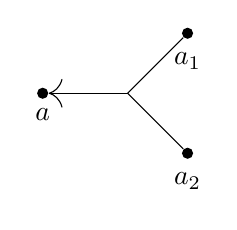
\begin{tikzpicture}[transform shape, every node/.style={circle, fill=black!100, inner sep=0.05cm}]
                \node[anchor=center, label=below:{$a$}](a){};
                \coordinate[right=1cm of a](ax);
                \node[above right=1cm of ax, label=below:{$a_1$}](a1){};
                \node[below right=1cm of ax, label=below:{$a_2$}](a2){};
                \draw[-{>[scale=2]}] (ax) -- (a);
                \draw[-] (a1) -- (ax) -- (a2);
            \end{tikzpicture}
            \caption*{Output edge $\langl a, a_1, a_2\rangl_o$}
        \end{subfigure}
        \begin{subfigure}{0.4\linewidth}
            \centering
            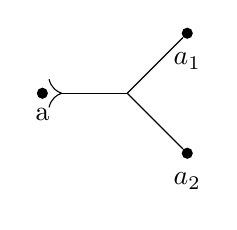
\begin{tikzpicture}[transform shape, every node/.style={circle, fill=black!100, inner sep=0.05cm}]
                \node[anchor=center, label=below:{a}](a){};
                \coordinate[right=1cm of a](ax);
                \node[above right=1cm of ax, label=below:{$a_1$}](a1){};
                \node[below right=1cm of ax, label=below:{$a_2$}](a2){};
                \draw[-{<[scale=2]}] (ax) -- (a);
                \draw[-] (a1) -- (ax) -- (a2);
            \end{tikzpicture}
            \caption*{Input edge $\langl a, a_1, a_2\rangl_i$}
        \end{subfigure}
    \end{figure}

    This is analogous to an input or output solo $u \, \tilde{x}$ in the calculus, where $a$ is $u$ or $\bar{u}$ and $a_1 \ldots a_n$ is $\tilde{x}$ as written in Definition~\ref{solo-calculus-syntax}.
    The intuition here is to define such an object within the diagrams for each type of agent in the calculus.
    Note that inputs and outputs must have matching arity --- a 2-arity input cannot communicate with a 3-arity output for obvious reasons.

    \begin{definition}{Box\\}
        A box is defined to be:
        \begin{align*}
            B \defeq \, \langl G, S \rangl \quad \text{for } S \subset nodes(G)\footnotemark
        \end{align*}\footnotetext{This is written as shorthand for all nodes contained within a given object, in this case $\{a \text{ s.t. } a \in nodes(S),\, S \in G \}$}
        where G is a \textit{graph} (or multiset of \textit{edges}) and S is a set of \textit{nodes}, referred to as the \textit{internal nodes} of $B$.
        The \textit{principal nodes} of $B$ are then $nodes(G) \setminus S$.
    \end{definition}

    \begin{figure}[H]
        \centering
        \begin{subfigure}{0.4\linewidth}
            \centering
            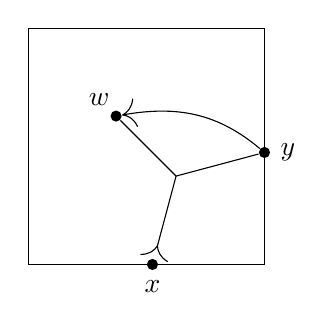
\begin{tikzpicture}[transform shape, every node/.style={circle, fill=black!100, inner sep=0.05cm}]
                \coordinate[anchor=center](nw);
                \coordinate[below=3cm of nw](sw);
                \coordinate[right=3cm of nw](ne);
                \coordinate[below right=3cm and 3cm of nw](se);
                \draw[-] (nw) -- (ne) -- (se) -- (sw) -- (nw);
                \node[right=1.5cm of sw, label=below:{$x$}](x){};
                \node[below=1.5cm of ne, label=right:{$y$}](y){};
                \node[below right=1.5cm of nw, label=above left:{$w$}](w){};
                \coordinate[below right=1cm of w](wxyx){};
                \draw[-] (y) -- (wxyx) -- (w);
                \draw[-{<[scale=2]}] (wxyx) -- (x);
                \draw[-{>[scale=2]}] (y) to [out=140, in=10] (w);
            \end{tikzpicture}
            \caption*{Box representing $!(w)(x \, w y \; | \; \tilde{w} \, y)$}
        \end{subfigure}\footnotemark
    \end{figure}\footnotetext{Usually the $w$ in the diagram would be excluded, but is included here for illustration purposes only.}

    This can then be seen to be analogous to the replication operator, with the idea being that the principal nodes form the perimeter of a box and cannot be replicated --- they serve as the interface to the internals of the box.

    \begin{definition}{Diagram\\}
        A solo diagram is defined to be:
        \begin{align*}
            SD \defeq (G, M, \ell)
        \end{align*}
        where $G$ is a finite multiset of \textit{edges}, $M$ is a finite multiset of \textit{boxes} and $\ell$ a labelling of the $nodes(G)$ and of $principals(M)$.
    \end{definition}
    
    From here, we can convert Solo Calculus to Diagrams, where composition is intuitively just including two separate diagrams together and scope is simply any connected nodes labelled by $\ell$.
    There are then four required reduction cases (edge-edge, edge-box, box-box and box internals) which can be deduced from the definition of the calculus.

    \begin{definition}{Diagram Reduction\\}
        Let $G, G_1, G_2 \ldots$ be arbitrary graphs, $M, M'$ arbitrary box multisets, $\alpha \defeq \langl a, a_1 \ldots a_k\rangl_i$, $\beta \defeq \langl a, a_1' \ldots a_k'\rangl_o$, $\sigma \defeq a_i \mapsto a_i'$, $\rho$ a arbitrary but fresh relabelling and $G\sigma$ shorthand for $\sigma(G) \defeq G\{dom(\sigma) / ran(\sigma)\}$ the application of the renaming $\sigma$ on the edges of G.
        $\alpha$ and $\beta$ need not be fixed to input and output respectively, but must be opposite parity.
        Then, the following reductions may be made:
        \begin{align*}
            (G \cup \{\alpha, \beta\}, M, \ell)                                                                             & \rightarrow (G\sigma, M\sigma, \ell') \\
            (G_1 \cup \{\alpha\}, M \defeq \langl G_2 \cup \{\beta\}, S\rangl, \ell)                                        & \rightarrow ((G_1 \cup G_2\rho)\sigma, M\sigma, \ell') \\
            (G, M \defeq \{\langl \{ \alpha \} \cup G_1, S_1\rangl,\langl \{ \beta \} \cup G_2, S_2\rangl\} \cup M', \ell)    & \rightarrow ((G \cup G_1\rho \cup G_2\rho)\sigma, M\sigma, \ell') \\
            (G, M \defeq \langl \{ \alpha, \beta \} \cup G_1, S\rangl \cup M', \ell)                                          & \rightarrow ((G \cup G_1\rho)\sigma, M\sigma, \ell')
        \end{align*}
        where each represents reduction of an edge-edge, edge-box, box-box and of box internals respectively.
    \end{definition}

    \begin{example*}
        \begin{figure}[H]
            \centering
            \begin{subfigure}{0.4\linewidth}
                \centering
                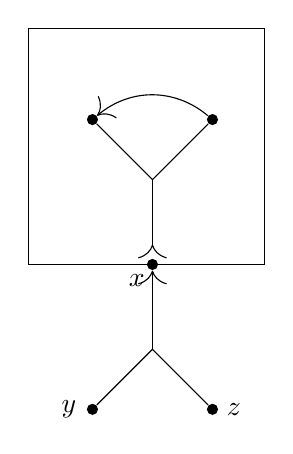
\begin{tikzpicture}[transform shape, every node/.style={circle, fill=black!100, inner sep=0.05cm}]
                    \coordinate[anchor=center](nw);
                    \coordinate[below=3cm of nw](sw);
                    \coordinate[right=3cm of nw](ne);
                    \coordinate[below right=3cm and 3cm of nw](se);
                    \draw[-] (nw) -- (ne) -- (se) -- (sw) -- (nw);
                    \node[right=1.5cm of sw, label=below left:{$x$}](x){};
                    \coordinate[below=1cm of x](xba){};
                    \coordinate[above=1cm of x](xaa){};
                    \node[above left=1cm of xaa](v){};
                    \node[above right=1cm of xaa](w){};
                    \node[below left=1cm of xba, label=left:{$y$}](y){};
                    \node[below right=1cm of xba, label=right:{$z$}](z){};
                    \draw[-{<[scale=2]}] (xaa) -- (x);
                    \draw[-{>[scale=2]}] (xba) -- (x);
                    \draw[-{>[scale=2]}] (w) to [out=140, in=40] (v);
                    \draw[-] (w) -- (xaa) -- (v);
                    \draw[-] (y) -- (xba) -- (z);
                \end{tikzpicture}
                \caption*{$\bar{x}\, y \, z \; | \; !(u \, v)(x \, u \, v \; | \; \bar{u} \, v)$}
            \end{subfigure}
            $\longrightarrow$
            \begin{subfigure}{0.4\linewidth}
                \centering
                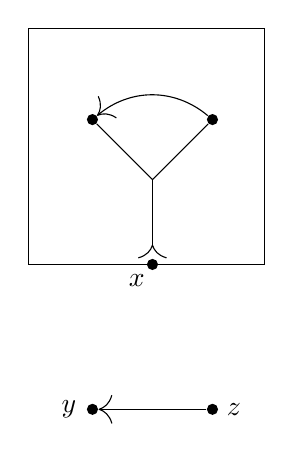
\begin{tikzpicture}[transform shape, every node/.style={circle, fill=black!100, inner sep=0.05cm}]
                    \coordinate[anchor=center](nw);
                    \coordinate[below=3cm of nw](sw);
                    \coordinate[right=3cm of nw](ne);
                    \coordinate[below right=3cm and 3cm of nw](se);
                    \draw[-] (nw) -- (ne) -- (se) -- (sw) -- (nw);
                    \node[right=1.5cm of sw, label=below left:{$x$}](x){};
                    \coordinate[below=1cm of x](xba){};
                    \coordinate[above=1cm of x](xaa){};
                    \node[above left=1cm of xaa](v){};
                    \node[above right=1cm of xaa](w){};
                    \node[below left=1cm of xba, label=left:{$y$}](y){};
                    \node[below right=1cm of xba, label=right:{$z$}](z){};
                    \draw[-{<[scale=2]}] (xaa) -- (x);
                    \draw[-{>[scale=2]}] (w) to [out=140, in=40] (v);
                    \draw[-] (w) -- (xaa) -- (v);
                    \draw[-{>[scale=2]}] (z) -- (y);
                \end{tikzpicture}
                \caption*{$\bar{y} \, z \; | \; !(u \, v)(x \, u \, v \; | \; \bar{u} \, v)$}
            \end{subfigure} 
        \end{figure}
    \end{example*}

    \begin{remark*}
        The graph objects associated with Solo Diagrams are particularly similar to bigraphs.
        These are a combination of a (possibly cyclic) `link graph' and a (strictly acyclic) `place graph', where the collection of nodes and edges forms the former and the subgraphs within boxes dictate the latter.
        Despite these two similar areas of research, including overlapping research by~\cite{bigraphs-pervasive-calculus}, it is found to be less relevant for this topic.
    \end{remark*}

 %% TODO: Probably improve, logical intuition to construction of diagrams
        ~\\ %% TODO: Summary/conclusion of lit review
        The Solo calculus is found to be simple, expressive and remarkable in its capability to be visualised as a diagram.
        For further reading,~\cite{acyclic-solos} present in great detail the topics of the $\pi$- and Solo calculus, Solo diagrams and furthermore differential interaction nets.

    %% TODO: Requirements

    \section{Technology}
        \subsection{Graph Visualisation}

    The system as a whole is planned to be implemented in the Python language, chosen for its ease of use and ability to be written in both a functional and object-oriented style, with each style likely suited to calculus and diagram implementation respectively.
    This being said, Python is seen as likely unsuitable for diagram visualisation and as such other solutions are mentioned here.\\
    
    \begin{definition*}{(Nice Diagrams)\\}
        For the output of diagrams by a system, it is seen as desirable to create `nice diagrams'.
        Some obvious requirements are:
        \begin{itemize}
            \item Fills the given space evenly
            \item Minimal overlap of edges and of nodes
            \item Lengths of edges are consistent
            \item Diagram will adapt as the graph changes
        \end{itemize}
        Here, `nice diagrams' is found to be mostly equivalent to springy force-directed diagrams such that addition or subtraction of parts of the graph, or manual manipulation of position, still leaves a graph that has nodes distributed evenly.
    \end{definition*}


    \begin{examples}
        The implementation of a solution to such a problem is complicated and performance-intensive, so is seen outside of the scope of this project.
        Instead, there exist several software libraries capable of producing these kind of outputs.
        Notable mentions include:
        \begin{itemize}
            \item \textit{GraphViz} for C~\footnotemark
            \item \textit{igraph} for C~\addtocounter{footnote}{-1}\footnotemark
            \item \textit{springy.js} for JavaScript
            \item \textit{VivaGraph.js} for JavaScript
            \item \textit{d3.js} for JavaScript
        \end{itemize}
    \end{examples}\footnotetext{These both have many language-specific APIs, so can be used from multiple languages and environments. The original library and interface is however written in C.}

    
    \begin{remarks}
        Most of these libraries, especially those that allow interactivity with the output, are written with the web-browser in mind and are subsequently written in JavaScript as the popular choice.
        With this in mind, this project is likely to focus on the use of the latter-mentioned \textit{d3.js}, which produces an interactive output or SVG from a JSON source.
        The reasoning for this choice is based upon both the features available and the relative maturity of the library.
        The popularity of the library across a large number of people, coupled with a development history dating back to early 2011.
    \end{remarks}
 %% TODO: Improve
        %% TODO: Section on programming languages used?

    \section{Solo Calculus}
        The implementation here was divided into two parts: a collection of objects and functions and a read-eval-print-loop (REPL) interface.
The former handles reduction strategies, string formatting of terms and the underlying data structure.
The latter handles user input and output, wrapping the objects and functions in a human-useable manner.

        \subsection{Calculus Implementation}\label{ssec:calculus-implementation}
    
    \subsubsection{Overview and Analysis}\label{sssec:calculus-analysis}
        The implementation of reduction semantics and calculus objects was achieved through converting all expressions to a canonical normal form.
        Due to the equivalence properties of the null agent $0$, it was excluded from the implementation as unnecessary.
        First, we must gather some possible structural congruences.

        \begin{lemma}{Structural Equivalence\\}
            For any agents $P, Q, \ldots$ the following structural equivalences hold.
            \begin{align*}
                (x)(y) P                & \equiv (x \, y) P \\
                P \; | \; (Q \; | \; R) & \equiv P \; | \; Q \; | \; R \\
                P \; | \; (x) Q         & \equiv (z)(P \; | \; Q\{z / x\}) \quad \text{where} \quad z \notin names(P) \cup names(Q)
            \end{align*}
            Using these congruences, expressions may be freely reordered through $\alpha$-equivalence only.
        \end{lemma}

        \begin{lemma}{Flattening Theorem\\}\label{flattening-theorem}
            For any agents $P, Q$ the following (non-structural) equivalence holds.
            \begin{align*}
                !(\tilde{x})(P \; | \; !Q) \sim (z)(!(\tilde{x})(P \; | \; z \, \tilde{y}) \; | \; !(\tilde{w})(\bar{z} \, \tilde{w} \; | \; Q\{\tilde{w}/\tilde{y}\})) \quad \text{where} \quad \tilde{y} \defeq fn(Q) \supset \tilde{x}
            \end{align*}
        \end{lemma}
        \begin{corollary*}{Non-Nesting of Replicators\\}
            By induction on $Q$ in Lemma~\ref{flattening-theorem}, any nesting of replicated agents may be flattened to a composition of non-nested replicators.
        \end{corollary*}
        This equivalence amounts to communicating between $P$ and $Q$ each bound name, allowing the two agents to `interact' within their shared scope, $\tilde{y}$ and $\tilde{w}$ respectively, without nesting replications.

        \begin{definition}{Normal Form\\}
            An agent $P$ is of normal form \textit{iff}
            \begin{align*}
                                    P \quad &\defeq \quad (\tilde{x})(\prod_{i}{y_i \, \tilde{z_i}} \; | \; \prod_{j}{! \, Q_j}) \\
                \text{where} \quad Q_j \quad &\defeq \quad (\tilde{x})(\prod_{k}{y_k \, \tilde{z_k}})
            \end{align*}
            That is, P is written as a 3-tuple of a scope, a composition of solos and a composition of replicators, where each replicator is written as a 2-tuple of a scope and a composition of solos only.
        \end{definition}

        \begin{lemma}{~\\}
            For any agent P, $\exists \, Q \sim P$ such that Q is in normal form.
            \begin{proof}
                The proof is trivial by applying recursively the equivalences above.
                See below for an algorithm for such a construction.
            \end{proof}
        \end{lemma}

        \begin{breakablealgorithm}
            \caption{Construction of Normal Forms}
            \begin{algorithmic}[1]
                \Require{Agent $P$ a Normal Form, $Q$ non-Normal Form}
                \Ensure{Agent $P'$, Normal Form of $P$ and $Q$}
                \Function{Normalise}{$P$}
                    \If{$Q$ a Scope}
                        \State$(\tilde{bn})Q' \defeq Q$
                        \State$collisions \defeq \tilde{bn} \cap names(P)$
                        \If{$collisions \neq \emptyset$}
                            \State$\alpha : collisions \rightarrow fresh\;names$
                            \State\Return\Call{Normalise}{$P$, $\alpha(Q)$}
                        \Else
                            \State\Return$(\tilde{bn})$\Call{Normalise}{$P$, $Q'$}
                        \EndIf\\

                    \ElsIf{$Q$ a Composition}
                        \State$Q_1 \;|\; \ldots \;|\; Q_n \defeq Q$
                        \State\Return\Call{Reduce}{\texttt{Normalise}, $P$, $Q_1 \ldots Q_n$}\\

                    \ElsIf{$Q$ a Replication}
                        \State$Q' \defeq$~\Call{Normalise}{$Q''$} where $!Q'' \defeq Q$
                        \If{$replicators(Q') \neq \emptyset$}
                            \State$\bar{Q} \defeq$~\Call{Flatten}{Q}
                            \State\Return\Call{Normalise}{$P$, $\bar{Q}$}
                        \Else
                            \State$collisions \defeq bn(P) \cap bn(Q')$
                            \State$\alpha : collisions \rightarrow fresh\;names$
                            \State\Return$P \; | \; !\,\alpha(Q')$
                        \EndIf\\

                    \ElsIf{$Q$ a Solo}
                        \State$(\tilde{bn})P' \defeq P$
                        \State$collisions \defeq \tilde{bn} \cap names(Q)$
                        \If{$collisions \neq \emptyset$}
                            \State$\alpha : collisions \rightarrow fresh\;names$
                            \State\Return\Call{Normalise}{$\alpha(P)$, $Q$}
                        \Else
                            \State\Return$(\tilde{bn})(P' \; | \; Q)$
                        \EndIf
                    \EndIf
                \EndFunction
            \end{algorithmic}
        \end{breakablealgorithm}
        Normalisation is then performed on an agent $P$ by $\texttt{Normalise}(P) \defeq \texttt{Normalise}(0, P)$.
        It will be seen later that this is exactly equivalent to how Solo Diagrams are represented.
        To ease implementation difficulties later on, the replicators of any normal form are subject to Barendregt's variable naming convention.
        That is, for $P \defeq (\tilde{x})(u \, \tilde{y} \; | \; \ldots \; | \; !Q)$, the bound names of $Q$ are free in $P \setminus !Q$.
        From here onwards, it is assumed that any agent has already been converted to normal form where appropriate.\\

        The algorithm for reductions is a simple search problem for two solos of matching subject and arity (number of names) and opposite parity (input vs. output).
        \begin{breakablealgorithm}
            \caption{Reduction of Solos}
            \begin{algorithmic}[1]
                \Require{Agent $P$}
                \Ensure{Agent $P'$, a reduction of $P$}
                \Function{Reduce}{$P$}
                    \ForEach{$i \in inputs(P)$}
                        \ForEach{$o \in outputs(P)$}
                            \If{$i$ agrees with $o$}
                                \State$\sigma \defeq$ \Call{Fuse}{$i$, $o$, $bn(P)$}
                                \If{$\sigma \neq \textit{none}$}
                                    \State\Return$\sigma(P - \{i, o\})$
                                \EndIf
                            \EndIf
                        \EndFor
                    \EndFor
                    \State\Return$P$
                \EndFunction
            \end{algorithmic}
        \end{breakablealgorithm}

        The next step is to find a suitable $\sigma$, should one exist. This is a renaming of the names of $P$ and must satisfy:
        \begin{align*}
            \sigma : \; & bn(P) \rightarrow names(P) \\
            \emptyset = \; & domain(\sigma) \cap range(\sigma) \\
            \sigma(x) = \; & y \implies \text{$x$ and $y$ have been fused}
        \end{align*}

        This is found through converting the list of pairs of object names to edges of a graph.
        For each disconnected subgraph, or partition, the span of names forms a set which must all be fused into one another.
        Subsequently, there must be at most one free name in this set as two or more would require renaming one free name to another, which is not allowed.
        If no free name exists, a bound name is chosen as the `free name' at random.
        $\sigma$ is then constructed by $\sigma(bn) \defeq fn$.

        \begin{breakablealgorithm}
            \caption{Fusion of Solos}
            \begin{algorithmic}[1]
                \Require{$i_1 \ldots i_n \text{ objects of solo } i, \quad o_1 \ldots o_n \text{ objects of solo } o, \quad bn \; \text{set of bound names}$}
                \Ensure{$\sigma : bn \rightarrow names(i) \cup names(o)$ or \textit{none}}
                \Function{Fuse}{$i_1 \ldots i_n$, $o_1 \ldots o_n$, $bn$}
                    \State$\texttt{Graph} \; g \defeq \{(i_j, o_j) \; | \; 1 \leq j \leq n\}$
                    \State$\texttt{Map} \; \sigma \defeq id$
                    \ForEach{$\texttt{Graph} \; \bar{g} \in partitions(g)$}
                        \State$isect \defeq nodes(\bar{g}) - bn$
                        \If{$|isect| = 0$}
                            \State$fn \defeq x \in nodes(\bar{g})$
                        \ElsIf{$|isect| = 1$}
                            \State$fn \defeq x \in isect$
                        \Else
                            \State\Return\textit{none}
                        \EndIf
                        \ForEach{$name \in nodes(\bar{g}) - \{fn\}$}
                            \State$\sigma(name) \defeq fn$
                        \EndFor
                    \EndFor
                    \State\Return$\sigma$
                \EndFunction
            \end{algorithmic}
        \end{breakablealgorithm}
        
        \begin{examples}{~\\}
            The following serve as a visualisation on the graphs constructed for finding a given $\sigma$.
            \begin{figure}[H]
                \centering
                \begin{tikzpicture}[transform shape, every node/.style={circle, fill=black!100, inner sep=0.05cm}]
                    \coordinate[anchor=center](center);
                    \coordinate[left=2cm of center](centerleft);
                    \node[left=0.86cm of centerleft, label=left:{$a$}](a){};i
                    \node[above=0.5cm of centerleft, label=above:{$b$}](b){};
                    \node[below=0.5cm of centerleft, label=below:{$c$}](c){};
                    \draw[-] (a) -- (b) -- (c) -- (a);
                    
                    \node[above=0.5cm of center, label=above:{$d$}](d){};
                    \node[below=0.5cm of center, label=below:{$f$}](f){};
                    \draw[-] (d) -- (f);

                    \coordinate[right=2cm of center](centerright);
                    \node[above=0.5cm of centerright, label=above:{$e$}](e){};
                    \node[below=0.5cm of centerright, label=below:{$g$}](g){};
                    \draw[-] (e) -- (g);
                \end{tikzpicture}
                \caption*{$\texttt{Fuse}((a, b, c, d, e), \; (b, c, a, f, g)) \rightarrow \{\{a, b, c\}, \{d, f\}, \{e, g\}\}$}
            \end{figure}
            \begin{figure}[H]
                \centering
                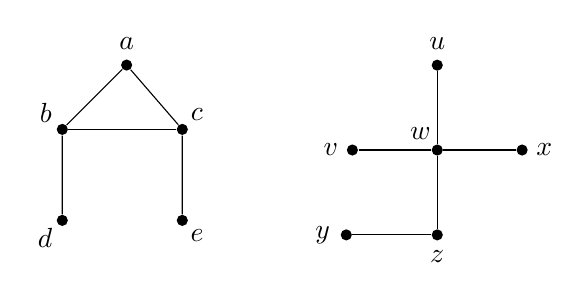
\begin{tikzpicture}[transform shape, every node/.style={circle, fill=black!100, inner sep=0.05cm}]
                    \coordinate[anchor=center](center);
                    \coordinate[below=0.5cm of center](fudgefactor);
                    \coordinate[left=2cm of fudgefactor](centerleft);
                    \node[above left=1cm of centerleft, label=above left:{$b$}](lal){};
                    \node[above right=1cm of centerleft, label=above right:{$c$}](lar){};
                    \node[below=1cm of lal, label=below left:{$d$}](lbl){};
                    \node[below=1cm of lar, label=below right:{$e$}](lbr){};
                    \node[above right=1cm of lal, label=above:{$a$}](lac){};
                    \draw[-] (lbl) -- (lal) -- (lac) -- (lar) -- (lbr);
                    \draw[-] (lar) -- (lal);

                    \coordinate[right=2cm of center](centerright);
                    \node[label=above left:{$w$}](rc) at (centerright) {};
                    \node[above=1cm of centerright, label=above:{$u$}](ra){};
                    \node[left=1cm of centerright, label=left:{$v$}](rl){};
                    \node[right=1cm of centerright, label=right:{$x$}](rr){};
                    \node[below=1cm of centerright, label=below:{$z$}](rb){};
                    \node[left=1cm of rb, label=left:{$y$}](rbl){};
                    \draw[-] (ra) -- (rc) -- (rb) -- (rbl);
                    \draw[-] (rl) -- (rc) -- (rr);
                \end{tikzpicture}
                \caption*{$\texttt{Fuse}((a, a, u, b, b, c, v, w, w, y), \; (b, c, w, c, d, e, w, x, z, z)) \rightarrow \{\{a, b, c, d, e\}, \{u, v, w, x, y, z\}\}$}
            \end{figure}
        \end{examples}

        This forms a complete implementation of non-replicating parts of the calculus.
        To avoid the implementation problems with replicators mentioned by~\cite{solo-diagrams}, it is necessary to only perform expansions on replicators that can be reduced.
        While the method described in the aforementioned paper would be suitable, it is enough to simply search for replicators which may be reduced, but only expand them rather than perform a complete reduction.
        This eases some implementation details and minimises code duplication while remaining correct.
        The expansion will be reduced on the next pass of the \texttt{Reduce} function.
        Below shows an extension of the \texttt{Reduce} function for a replicator-replicator fusion (reduction of the form $!P \;|\; !Q$).

        \begin{breakablealgorithm}
            \caption{Reduction of Replicators}
            \begin{algorithmic}[1]
                \Require{Agent $P$}
                \Ensure{Agent $P'$, a reduction of $P$}
                \Function{Reduce}{$P$}
                    \ForEach{$i \in inputs(P)$}
                        \State$\ldots$
                    \EndFor\\

                    \ForEach{$i \in inputs(R_i) \; | \; R_i \in \bigcup_{!R \in P} R$}
                        \ForEach{$o \in outputs(R_o) \; | \; R_o \in \bigcup_{!R \in P} R$}
                            \If{$i$ agrees with $o$}
                                \State$\sigma \defeq$ \Call{Fuse}{$i$, $o$, $bn(P) \cup bn(R_i) \cup bn(R_o)$}
                                \If{$\sigma \neq \textit{none}$}
                                    \State\Return$P \cup \{R_i \; | \; R_o\}$
                                \EndIf
                            \EndIf
                        \EndFor
                    \EndFor
                    \State\Return$P$
                \EndFunction
            \end{algorithmic}
        \end{breakablealgorithm}

        The third case of solo-replicator fusion (reduction of the form $P \;|\; !Q$) is then trivial.


    \subsubsection{Testing and Correctness}
        Testing of this section was integrated with testing of the REPL by using the helper functions it provided for constructing agents.
        An in-depth description can be found in~\ref{sssec:repl-testing}. \\
        
        Early tests could be tested by string equalities and this was sufficient.
        More complicated agents however led to non-deterministic results and non-trivial equalities.
        The first example of this occured while comparing the following agents:
        \begin{align*}
            (x) p \, x \quad\equiv\quad (y) p \, y \quad\neq\quad (x) p \, y
        \end{align*}
        Before testing could be achieved in an automated manner, an algorithm for testing for $\alpha$-equivalence was first required.\\

        It will be seen later that conversion of calculus expressions into diagrams intuitively shows $\alpha$-equivalence is reducible to graph isomorphism, so is expected to be of poor performance.
        \begin{breakablealgorithm}
            \caption{$\alpha$-Equivalence of Agents}
            \begin{algorithmic}[1]
                \Require{Agents $P, Q$}
                \Ensure{Map $\alpha : names(P) \rightarrow names(Q) \textit{ s.t. } \alpha(P) \equiv Q$ or \textit{none}}
                \Function{$\alpha$-Equivalence}{$P$, $Q$}
                    \If{$P \equiv Q$}
                        \State\Return$id$
                    \EndIf
                    \For{$comb_{scope} \in combinations(scope(P), scope(Q))$}
                        \State$\alpha_{P, Q} : x \mapsto y \; \forall \; (x, y) \in comb_{scope}$
                        \For{$comb_{replicator} \in combinations(\{R \; | \; !R \in P\}, \{R \; | \; !R \in Q\})$}
                            \ForEach{$(r_P, r_Q) \in comb_{replicator}$}
                                \State$\alpha_{r_P, r_Q} \defeq$ \Call{$\alpha$-Equivalence}{$r_P, r_Q$}
                            \EndFor
                            \If{$\textit{none} \in \{\alpha_{r_P, r_Q} | (r_P, r_Q) \in comb_{replicator}\}$}
                                \State\textbf{continue for}
                            \ElsIf{$\exists \; \alpha_1, \alpha_2 \in \{\alpha_{r_P, r_Q}\} \textit{ s.t. } \alpha_1 \text{ disagrees with } \alpha_2$}
                                \State\textbf{continue for}
                            \Else
                                \State$\alpha \defeq \alpha_{P, Q} \cup \bigcup_{\alpha \in \{\alpha_{r_P, r_Q}\}} \alpha$
                            \EndIf
                            \If{$\alpha(P) \equiv \alpha(Q)$}
                                \State\Return$\alpha$
                            \EndIf
                        \EndFor
                        \If{$\alpha(P) \equiv \alpha(Q)$}
                            \State\Return$\alpha$
                        \EndIf
                    \EndFor
                    \State\Return\textit{none}
                \EndFunction
            \end{algorithmic}
        \end{breakablealgorithm}
        Note that the algorithm here does not take into account parity of subjects.
        While parities of free subject names do affect $\alpha$-equivalence, those of bound subject names may be reversed.
        That is, while $u \, x \neq \bar{u} \, x$, it does hold that $(u)u \, x \equiv (u)\bar{u} \, x$.


    \subsubsection{Discussion}
        The initial implementation stayed closer to the core concepts of the calculus.
        There existed separate classes of objects for each of Scopes, Compositions, Replications, Matches and Solos.
        While such an approach is perhaps more intuitive, problems arise due to conflicts between how the data structure naturally appears to be tree-like where properties of agents are functions of themselves and their children only and how whether or not a name is bound or free is a property dependent upon an agent or its parent, grandparent etc.

        \begin{example*}
            Consider the following equivalent expressions.
            \begin{align*}
                P \quad & \defeq \quad (y)(a \, x \,|\, (\bar{a} \, y \,|\, p \, y)) \\
                Q \quad & \defeq \quad (a \, x \,|\, (y)(\bar{a} \, y \,|\, p \, y))
            \end{align*}
            Both $P$ and $Q$ have the property that $y$ is a bound name and both should reduce to the term $p \, x$.
            In both cases, $y$ and $x$ are fused into the free name $x$. The scope of $y$ disappears and the remaining $p$ term, which may be thought of as a `print' instruction, displays the result of the fusion.
            Consider now the (inequivalent) expression.
            \begin{align*}
                R \quad & \defeq \quad (a \, x \; | \; (y)\bar{a} \, y \; | \; p \, y)
            \end{align*}
            This term, while similar to $P$ and $Q$, reduces to the term $p \, y$, as our scoped $y$ that is fused is not the same as the free $y$ that is `printed'.
            This can be seen through $\alpha$-equivalence and renaming $(y)\bar{a} \, y$ to the equivalent term $(z)\bar{a} \, z$ and observing that $a$ is a fusion on $x$ and $z$.

            The distinction between the two behaviours is not intuitive, especially in non-trivial cases where agents may be deeply nested.
        \end{example*}

        The above example is further amplified when manipulating expressions symbolically.
        When searching for reducible patterns, the expression is divided and recombined, rearranging the expression tree and subsequently each node's parents.
        While the problem is solvable through updating which node has which parent as the expression is rearranged and manipulated, the solution eventually becomes an attempt to form a normal form out of the expression, leading to the revised method described in~\ref{sssec:calculus-analysis}.\\

        Through the implementation of the calculus, many interesting properties became apparent, with some of the most noticeable listed below.

        \begin{lemma*}{Non-Finite Reductions\\}
            There exist expressions for which reductions may be performed indefinitely.
            For a reduction to be non-finite, both solos must be replicable.
            In particular, expressions of the form $(!(\tilde{x})(u \, \tilde{x} \; | \; P) \; | \; !(\bar{u} \, \tilde{y} \; | \; Q) \; | \; R)$ are non-finite.
        \end{lemma*}

        \begin{example*}{~\\}
            Consider the following expressions, each a fusion of a bound $x$ and free $y$:
            \begin{align*}
                P \rightarrow P'\{y / x\} & \text{ where } x \in \; !(x)Q \in P \text{ and } y \in \; !R \in P \\
                (x)P \rightarrow P'\{y / x\} & \text{ where } x \in \; !Q \in P \text{ and } y \in \; !R \in P
            \end{align*}
            The first expression may be reduced indefinitely, each time adding the expansion of $Q$ to $P$.
            The second may be performed once, after which each $x$ in $Q$ is renamed to $y$.
            It is then ambiguous as to whether it may be performed again --- on one hand the fusion is on two free names, on the other the two names are the same, so there is only one distinct free name.
        \end{example*}

        \begin{remark*}{Behaviour of Trivial Reductions\\}
            For this body of work, since the reduction requires $\sigma : \emptyset \rightarrow \emptyset$, it was assumed that under such conditions a reduction should not be seen to have happened.
        \end{remark*}
 %% TODO: Barendregt variable convention, flattening theorem, α looks horrid but necessary
        \subsection{Read-Eval-Print-Loop}

    \subsubsection{Overview and Analysis}
        A simple REPL interface was constructed to interact with the code written in~\ref{ssec:calculus-implementation}.
        This was done using extended regular expressions similar to those found in the Perl programming language.
        These do not meet the normal definitions of regular expressions as they additionally support recursive matches, backreferences and various other syntactic additions that make them context-free grammars rather than regular expressions.
        In fact, given a suitable engine for applying context-free grammars, this would be a preferable way to parse expressions. \\

        For each agent, there was an extended regex matching its string representation, with backreferences to extract the necessary data.
        Each of $(?P\langl name \rangl \textit{expression})$ represents a named backreference to the given expression and $(? \, \& rec)$ is a recursive call to the outer $(?\langl rec \rangl \textit{expression})$ expression.
        
        \begin{definition}{Solo Matching\\}
            Solos are built using the regex as follows:
            \begin{align*}
                u \, \tilde{x}       & \quad \longleftarrow \quad \backslash s? (?P \langl subject \rangl [a-z \, 0-9]+) \backslash s (?P \langl objects \rangl ([a-z \, 0-9]+ \backslash s?)+) \backslash s? \\
                \bar{u} \, \tilde{x} & \quad \longleftarrow \quad \backslash s? \backslash ^{\wedge} (?P \langl subject \rangl [a-z \, 0-9]+) \backslash s (?P \langl objects \rangl ([a-z \, 0-9]+ \backslash s?)+) \backslash s?
            \end{align*}
            where a valid name is any lowercase alphanumeric word and $\bar{u}$ is inputted as \texttt{$^{\wedge}$u} and each of \texttt{subject} and \texttt{objects} represent the subject and objects of the solo respectively.
        \end{definition}

        \begin{definition}{Replication\\}
            Replicators are built using the regex as follows:
            \begin{align*}
                ! P \quad \longleftarrow \quad \backslash s? \; !(?P \langl agent \rangl.*)\backslash s?
            \end{align*}
            where \texttt{agent} represents $P$ for the expression $!P$.
        \end{definition}

        \begin{definition}{Scope\\}
            Scopes are built using the regex as follows:
            \begin{align*}
                (x)P \quad \longleftarrow \quad \backslash s? \backslash ((?P \langl bindings \rangl([a-z \, 0-9]+ \backslash s?)+)\backslash )(?P\langl agent \rangl[^{\wedge}\backslash s].+)\backslash s?
            \end{align*}
            where each of \texttt{bindings} and \texttt{agent} represent $x$ and $P$ respectively for the expression $(x) P$.
        \end{definition}

        \begin{definition}{Composition\\}
            Compositions are built using the recursive regex as follows:
            \begin{align*}
                P_1 \, | \ldots | \, P_n \quad \longleftarrow \quad & \backslash s? \backslash (?\langl agents\rangl~\texttt{R}+) (\backslash | (?\&agents))?)\backslash )\backslash s? \\
                \text{where} \quad \texttt{R} \quad \defeq \quad & (?\langl agent\rangl([^{\wedge}|()] | (?\langl rec\rangl\backslash ((?:[^{\wedge}()]++|(?\&rec))*\backslash )))
            \end{align*}
            where each \texttt{agent} is collected in \texttt{agents} and represents each of $P_1 \ldots P_n$.
        \end{definition}
        It is accepted that this is difficult to read and would benefit from a better-structured parsing system.
        For this project and as a write-once solution, it is suitable enough.


    \subsubsection{Testing and Correctness}\label{sssec:repl-testing}
        Testing was first done of the structural equivalence and equality of expressions.
        First, for each of the congruences described above, a normalised expression and its known normal form were tested for equality.
        Testing of reductions was done through testing each of the four cases of fusions being performed:
        \begin{itemize}
            \item Normal fusion $(\tilde{x})(a \tilde{x} \,|\, \bar{a} \, \tilde{y})$
            \item Cross-replicator fusion $(\tilde{x})(a \, \tilde{x} \,|\, !(\bar{a} \, \tilde{y}))$
            \item Multi-replicator fusion $(\tilde{x})(!(a \, \tilde{x}) \,|\, !(\bar{a} \, \tilde{y}))$
            \item Inter-replicator fusion $(\tilde{x})(!(a \, \tilde{x} \,|\, \bar{a} \, \tilde{y}))$
        \end{itemize} 
        where for each, there exist approximately four cases of which variables are bound and where the matching scope lies.
        %% TODO: Finally, a test of an expression containing all of the above agents was reduced and checked for correctness.

        Due to the open-endedness of the problem, it is difficult to provide a conclusive, complete testing suite.
        In particular, checking for false positives presents a large space of possible tests.
        This was managed by reducing to the above unit tests and combining with the integration test of each case of fusion.\\

        A sample of test outputs can be found in~\ref{ssec:appendix-calculus-tests}


    \subsubsection{Discussion}
        No research was done as to the usability of this interface.
        Future work would vastly improve the description provided here, particularly with regards to error-reporting.
        Another notable flaw is a disconnect between text inputted and outputted, for example \textit{$^{\wedge}$p a b c} $\rightarrow$ \textit{$\bar{p}$ a b c}.\\

        With further work on the project, I would have hoped to embed this REPL interface in the REST server described in~\ref{ssec:rest-server}.
        Through this, the diagram presented by the server could be changed on the server-side.
 %% TODO: Subject parity in alpha equivalence

    \section{Solo Diagrams}
        The implementation here was divided into two parts: a collection of objects and functions and a read-eval-print-loop (REPL) interface.
The former handles reduction strategies, string formatting of terms and the underlying data structure.
The latter handles user input and output, wrapping the objects and functions in a human-useable manner.

        \subsection{Results}

\subsection{Objects, Functions and Datatypes}

\subsection{REST Server}

        \subsection{Visualiser and REST Server}\label{ssec:rest-server}

    \subsubsection{Overview and Analysis}
        Diagrams produced by the above sections were visualised as graphs of nodes and edges within an SVG (scalable vector graphic).
        Further, this graph was made interactive using ECMAScript's d3.js library, in particular using force-directed graphs.
        This was coupled through a back-end server acting as a reduction engine with a representational state transfer (REST) architecture and a front-end webpage with ECMAScript components for interacting with the output of the server.\\

        The REST server was a single endpoint with options of GET and POST requests.
        GET returned an example diagram as a JSON object --- in particular, this was a collection of four disconnected diagrams, one for each type of edge reduction.
        POST would, given a JSON object, reduce and return a new diagram.
        
        \begin{remark*}{Cross-Origin Resource Sharing (CORS)\\}
            As a note on the bureaucracy of various web standards, the implementation written for this project involved making cross-origin HTTP requests.
            By default, this behaviour is not allowed, so an additional CORS layer is wrapped around the server to allow such requests.
        \end{remark*}~

        The front-end visualisation was, in comparison, far more complex.
        To begin, there would be a GET request to the REST server for the default diagram.
        The returned JSON object was parsed to an SVG.
        In particular, SVG groups were made of edges, nodes and boxes.
        Each class of edge, node and box contained a set of polylines, a circle and a collection of both nodes and edges respectively.
        Nodes were coloured depending upon the property of their position relative to boxes: external, perimeter or internal.\\

        Interactivity was added using an ECMAScript script and additionally a `Reduce' button.
        Each node was made draggable and forces were added to each node and edge.
        In particular:
        \begin{itemize}
            \item Edges were given spring forces to allow them to stretch on drag actions and contract to a relaxed length otherwise.
            \item Nodes were given repulsive charges to allow them to spread themselves out evenly over the available space.
            \item The graph as a whole was given a small central attractive charge to keep the graph centered in the viewing panel.
        \end{itemize}
        The `Reduce' button would then make a POST request to the REST server to update the current graph dataset with its reduction.\\

        Due to the odd paradigms of the language, as follows is a unformatted extract of the script used

        \begin{itemize}
            \item Nodes were tracked through reductions --- those not reduced inherited their position from the previous diagram, enforcing smoothness.
            \item Problems with nodes on perimeter of boxes --- as diagrams are defined as a collection  of edges, perimeter nodes are both internal and external nodes to a box.
        \end{itemize}


    \subsubsection{Testing and Correctness}
        Pictures~\ldots


    \subsubsection{Discussion}
        idk


    \section{Conclusion}
        \subsection{Summary}

\subsection{Concluding Statements}

\subsection{Future Work and Research}

\subsection{Further Reading}

 %% TODO: Consequences of choices made

    \section{References}
        \bibliography{dissertation}

    \section{Appendix}
        \subsection{Calculus Testing}\label{ssec:appendix-calculus-tests}
    Output of command \texttt{python src/calculus/tests.py}
    \small\verbatiminput{meta/calculus-tests.out}\normalsize

\subsection{Graph Visualisation Source Sample}\label{ssec:appendix-graph-source}
    Sample output of file \texttt{src/visualisation/graph.js}
    \small\verbatiminput{meta/graph-source.out}\normalsize

\subsection{Full Chain of Diagram Reductions}\label{ssec:appendix-diagram-reduction}
    Full reduction of the union of the examples in~\ref{sssec:diagram-reductions}

    \begin{figure}[H]
        \centering
        \begin{subfigure}{0.4\linewidth}
            \includegraphics[width=\textwidth]{diagrams/all-diagrams.png}
        \end{subfigure}
        $\longrightarrow$
        \begin{subfigure}{0.4\linewidth}
            \includegraphics[width=\textwidth]{diagrams/all-diagrams-r1.png}
        \end{subfigure}
        $\longrightarrow$
    \end{figure}

    \begin{figure}[H]
        \centering
        \begin{subfigure}{0.4\linewidth}
            \includegraphics[width=\textwidth]{diagrams/all-diagrams-r2.png}
        \end{subfigure}
        $\longrightarrow$
        \begin{subfigure}{0.4\linewidth}
            \includegraphics[width=\textwidth]{diagrams/all-diagrams-r3.png}
        \end{subfigure}
        $\longrightarrow$
    \end{figure}

    \begin{figure}[H]
        \centering
        \includegraphics[width=0.4\textwidth]{diagrams/all-diagrams-r4.png}
    \end{figure}


\end{document}
